\documentclass[aps,pre,floats,floatfix,twocolumn]{revtex4-1}
\RequirePackage{lineno} 
\renewcommand\thelinenumber{\color{red}\arabic{linenumber}}

%figs
\usepackage{graphicx} 
\usepackage{subcaption}
\captionsetup{singlelinecheck = false, format= hang, justification=raggedright, labelsep=space}
\usepackage{epstopdf}
\graphicspath{{./Figs/}}

%fonts
\usepackage{latexsym}
\usepackage{amsmath}
\usepackage{amssymb}
\usepackage{bm}
\usepackage{wasysym}

%more
\usepackage{ifthen}
\usepackage{color}
\usepackage[colorlinks,allcolors=blue,bookmarks=true]{hyperref}


%%%%%%%%%%%%%%%%%%%%%%%%%%%%%%%%%%%%%%%%%%%%%%%%%%%%%%%%%%%%%%%%

% Standard symbols 
\newcommand{\sinc}{\mbox{sinc}}
\newcommand{\const}{\mbox{const}}
\newcommand{\trc}{\mbox{trace}}
\newcommand{\intt}{\int\!\!\!\!\int }
\newcommand{\ointt}{\int\!\!\!\!\int\!\!\!\!\!\circ\ }
\newcommand{\ar}{\mathsf r}
\newcommand{\im}{\mbox{Im}}
\newcommand{\re}{\mbox{Re}}

% Special symbols
\newcommand{\mass}{\mathsf{m}} 
\newcommand{\Mass}{\mathsf{M}} 

% Math constractions
\newcommand{\tbox}[1]{\mbox{\tiny #1}}
\newcommand{\bmsf}[1]{\bm{\mathsf{#1}}} 
\newcommand{\amatrix}[1]{\begin{matrix} #1 \end{matrix}} 
\newcommand{\eexp}[1]{\mathrm{e}^{#1}}
\newcommand{\pd}[2]{\frac{\partial #1}{\partial #2}}
\newcommand{\bra}[1]{\left\langle #1 \right|}
\newcommand{\ket}[1]{\left| #1 \right\rangle}
\newcommand{\braket}[1]{ \left\langle #1 \right\rangle}
\newcommand{\Braket}[2]{ \left\langle #1 \middle| #2 \right\rangle}
\newcommand{\BraKet}[3]{ \left\langle #1 \middle| #2 \middle| #3 \right\rangle}
\newcommand{\avg}[1]{\left\langle #1 \right\rangle}
\newcommand{\ola}{\protect\overleftarrow}
\newcommand{\ora}{\protect\overrightarrow}
\newcommand{\commutator}[2]{\left[#1,#2\right]}

% Equations
%\newcommand{\be}[1]{\marginpar{\textcolor{red}{e#1}} %
\newcommand{\beq}{\begin{eqnarray}}
\newcommand{\eeq}{\end{eqnarray}} 

% Text arrangement
\newcommand{\hide}[1]{}
%\newcommand{\Eq}[1]{\textcolor{blue}{{Eq.}\!~(\ref{#1})}} 
\newcommand{\Eq}[1]{\textcolor{blue}{{Eq.}\!\!~(\ref{#1})}} 
\newcommand{\App}[1]{\textcolor{blue}{{Appendix}\!~#1}} %{\textcolor{blue}{{Appendix}\!~(\ref{#1})}} 
\newcommand{\Sec}[1]{\textcolor{blue}{{Section}\!~(\ref{#1})}}
\newcommand{\Fig}[1]{\textcolor{blue}{Fig.}\!\!~\ref{#1}}
\definecolor{myred}{rgb}  {0.5,0.0,0.0}
\newcommand{\rmrk}[1]{\textcolor{myred}{#1}}

\newcommand{\hrefl}[2]{\href{#2}{(#1)}}
\newcommand{\sect}[1]{{\bf #1.--}}
\newcommand{\drawline}{\begin{picture}(500,1)\line(1,0){500}\end{picture}}
\newcommand{\bitem}{$\bullet$ \ \ \ }
\newcommand{\Cn}[1]{\begin{center} #1 \end{center}}
%%%%%%%%%%%%%%%%%%%%%%%%%%%%%%%%%%%%%%%%%%%%%%%%%%%%%%%%%%%%
%%%%%%%%%%%%%%%%%%%%%%%%%%%%%%%%%%%%%%%%%%%%%%%%%%%%%%%%%%%%
\newcommand{\heading}[1]{\begin{center} {\Large {\bf } #1} \end{center}}
\newcommand{\auname}[1]{\begin{center} {\bf } #1 \end{center}}


%%%%%%%%%%%%%%%%%%%%%%%%%%%%%%%%%%%%%%%%%%%%%%%%%%%%%%%%%%%%%%%%

%counters
\renewcommand{\thesection}{\arabic{section}}
\renewcommand{\thesubsection}{\arabic{subsection}}
\renewcommand{\thesubsubsection}{\arabic{subsubsection}}
\setcounter{section}{0}
\setcounter{subsection}{0}

% Sections for research notes
\newcommand{\sectA}[1]
{
\addtocounter{section}{1}
\setcounter{subsection}{0}
\ \\
\pdfbookmark[2]{\thesection. \ #1}{sect.\thesection}
{\Large\bf $=\!=\!=\!=\!=\!=\;$ [\thesection] \ #1}
\nopagebreak
}

% Subsections for research notes
\newcommand{\sectB}[1]
{
\addtocounter{subsection}{1}
\ \\
\pdfbookmark[2]{\ \ \ \ \thesection.\thesubsection. \ #1}{subsect.\thesection.\thesubsection}
{\bf $=\!=\!=\!=\!=\!=\;$ [\thesection.\thesubsection] \ #1}
\nopagebreak
}

% Sections for lecture notes
\newcommand{\sheadA}[1]
{
\addtocounter{section}{1}
%
\newpage 
\begin{center} 
\pdfbookmark[1]{#1}{shdA\thesection}
%\hypertarget{shdA\thesection.1}{}
{\bf {\LARGE #1}} 
\end{center} 
%
\addtocontents{toc}{\protect\contentsline{section}{{\Large #1}}{}{}}
}

% SubSections for lecture notes
\newcommand{\sheadB}[1]
{
\addtocounter{subsection}{1}
\setcounter{subsubsection}{0} 
%
\vspace{5mm}
\pdfbookmark[2]{#1}{shdB\thesubsection}
{\bf\LARGE[\thesubsection] \ #1} 
\nopagebreak
%
\addtocontents{toc}{\protect\contentsline{subsection}{\thesubsection \ \ #1}{\thepage}{shdB\thesubsection.2}}
}

% SubSubSections for lecture notes
\newcommand{\sheadC}[1]
{
\addtocounter{subsubsection}{1}
%
\vspace{5mm}
{\Large\bf $=\!=\!=\!=\!=\!=\;$ [\thesubsection.\thesubsubsection] \ #1}  
\nopagebreak
}


% Page setup for notes
\onecolumngrid
\newlength{\Parskip}
%\newlength{\Mathskip}
\setlength{\Parskip}{0.3cm}
%\setlength{\Mathskip}{0cm}
\setlength{\parindent}{0cm}
%\setlength{\mathindent}{2cm}
\setlength{\parskip}{\Parskip}



%%%%%%%%%%%%%%%%%%%%%%%%%%%%%%%%%%%%%%%%%%%%%%%%%%%%%%%%%%%%%%%%%%%%%%%%%%%%%%%%%%%%%%%%%%%%%%%%%%%%%%%%%
%%%%%%%%%%%%%%%%%%%%%%%%%%%%%%%%%%%%%%%%%%%%%%%%%%%%%%%%%%%%%%%%%%%%%%%%%%%%%%%%%%%%%%%%%%%%%%%%%%%%%%%%%

%\renewcommand{\includegraphics}[2][]{\vspace*{4cm} {\color{blue} FIGURE (unccomment renewcommnd to display)} \ \\ \ }

%%%%%%%%%%%%%%%%%%%%%%%%%%%%%%%%%%%%%%%%%%%%%%%%%%%%%%%%%%%%%%%%%%%%%%%%%%%%%%%%%%%%%%%%%%%%%%%%%%%%%%%%%
%%%%%%%%%%%%%%%%%%%%%%%%%%%%%%%%%%%%%%%%%%%%%%%%%%%%%%%%%%%%%%%%%%%%%%%%%%%%%%%%%%%%%%%%%%%%%%%%%%%%%%%%%
\begin{document}
\font\myfont=cmr12 at 20pt
\title{\myfont Numerical Examination of Pulses in Mass-Conserving
Activator-Inhibitor Media\\ 
\vspace{0.5cm}
\large
Ben-Gurion University of the Negev  \\
        Faculty of Natural Sciences, Department of Physics \\}
\author{Submitted by: Ariel Falk \\Advisor: Arik Yochelis\\ }

\maketitle

\onecolumngrid
%%%%%%%%%%%%%%%%%%%%%%%%%%%%%%%%%%%%%%%%%%%%%%%%%%%%%%%%%%%%%%%%%%%%%%%%%%%%%%%%%%%%%%%%%%%%%%%%%%%%%%%%%
%%%%%%%%%%%%%%%%%%%%%%%%%%%%%%%%%%%%%%%%%%%%%%%%%%%%%%%%%%%%%%%%%%%%%%%%%%%%%%%%%%%%%%%%%%%%%%%%%%%%%%%%%
\sectA{Introduction}

Different natural systems, such as biological cells, chemical reactions and ecological populations exhibit mechanisms of excitable pulses. These pulses propagate in an excitable media and their signature behavior is that upon collision they annihilate each other. One of the most interesting mechanisms is of intracellular actin waves. Actin waves, which appear on cell membranes, demonstrate different outcomes upon collision. One of these outcomes is annihilation, which relates to excitable pulses. Yet, regarding actin waves, there are other behaviors as well. These behaviors will be discussed later. The importance of studying these waves and their nature may be due to the connection between them and the process of macropinocytosis [1]. In this process cells grow actin-based vertical protrusions (ruffles) that collapse or fold back on either themselves or the cell body. The collapse creates enclosed cavities that are then internalized as vesicles (macropinosomes). The extracellular fluid inside of macropinosomes contains, for example, dissolved macromolecules that serve the nutrition of cells. These protrusions perform as a type of actin wave, that is, a propagating wave-front of actin polymerization at the dorsal cell side.

\begin{figure}[hbt!]\centering
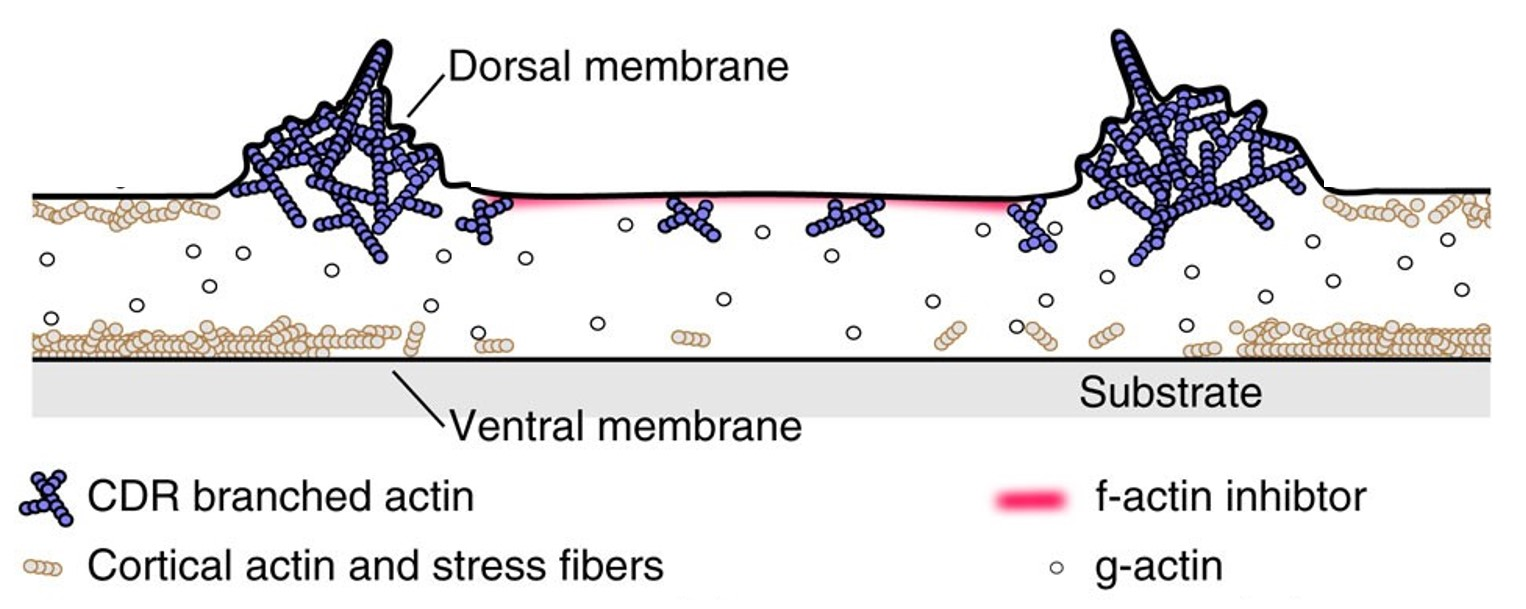
\includegraphics[scale=0.4]{actin wave.jpg}
\caption{\label{im1}Schematic sketch of the distribution of actin polymers, actin monomers and the inhibitor of actin polymerization in a cross section through a wavelike dorsal ruffle [1].} 
\end{figure}

In this project we examine a simplified, one-dimensional, reaction-diffusion model that describes the polymerization of actin and was formulated using a more complex circular dorsal ruffles model [1], as the similarity between the kinetics of the two phenomena is close .The purpose of this examination is to study different wave patterns that arise from this simplified model, through different numerical methods.
\newpage
%%%%%%%%%%%%%%%%%%%%%%%%%%%%%%%%%%%%%%%%%%%%%%%%%%%%%%%%%%%%%%%%%%%%%%%%%%%%%%%%%%%%%%%%%%%%%%%%%%%%%%%%%
%%%%%%%%%%%%%%%%%%%%%%%%%%%%%%%%%%%%%%%%%%%%%%%%%%%%%%%%%%%%%%%%%%%%%%%%%%%%%%%%%%%%%%%%%%%%%%%%%%%%%%%%%
\sectA{The model}

We start with a model of actin polymerization waves, adjusted from a model of circular dorsal ruffles that propagate on the dorsal side of the cell membrane [2]:
\beq
      \frac{\partial N}{\partial t}&=&\frac{N^2S}{1+I}-N+D_N\frac{\partial^2 N}{\partial x^2} \\\nonumber
      \frac{\partial S}{\partial t}&=&\frac{-N^2S}{1+I}+N+\frac{\partial^2 S}{\partial x^2} \\\nonumber
      \frac{\partial I}{\partial t}&=&k_NN-k_II+D_I\frac{\partial^2 I}{\partial x^2}
\eeq

Here N represents the polymerized actin filaments, S represents the actin monomers and I represents the actin polymerization inhibitor.

Next, we apply the forward Euler method in order to solve the equations numerically. To apply this method it is first needed to treat the $x$ and $t$ coordinates. We choose equally spaced points along the t and x axes such that:
\beq
    x_j&=&x_0+j{\Delta}x, \ \ \ j=0,1,...,J\\\nonumber
     t_n&=&t_0+n{\Delta}t,\ \ \ n=0,1,...,N
\eeq
The index $j$ represents the number of space steps and $n$ represents the number of time steps. Let $U^{n}_j$ denote $U(t_n,x_j)$. Now, each derivative will have the form:
\begin{eqnarray}
    \frac{\partial U}{\partial t}&=&\frac{U^{n+1}_j-U^{n}_j}{\Delta t}+O({\Delta}t)\\\nonumber
     \frac{\partial^2 U}{\partial x^2}&=&\frac{U^{n}_{j+1}+U^n_{j-1}-2U^{n}_j}{\Delta x^2}+O({\Delta}x^2)
\end{eqnarray}
It is important to notice that this method is simple, takes little storage and executes quickly, but it has stability problems. The model consists of a set of parabolic equations with a constant diffusion coefficient. To examine the stability problems of our model we use the von Neumann stability analysis. We imagine that the coefficients of the difference equations are slowly varying as to be considered constant in space and time. In that case, the independent solutions, or eigenmodes, of the difference equations are all of the form:
\beq
{U^{n}_j={\xi}^{n}e^{ikj{\Delta}x}}
\eeq
where $k$ is a real spatial wave number, which can have any value, and $\xi=\xi(k)$ is a complex number that depends on $k$.
The key fact is that the time dependence of
a single eigenmode is nothing more than successive integer powers of the complex number $\xi$. Therefore, the difference equations are unstable (i.e. have exponentially growing modes) if $|\xi|>1$ for some $k$. To find $\xi$ we substitute equation (8) into a basic diffusion equation of the form:
\beq
\frac{U^{n+1}_j-U^{n}_j}{\Delta t}&=&D\left[\frac{U^{n}_{j+1}+U^n_{j-1}-2U^{n}_j}{\Delta x^2}\right]
\eeq
This will lead to:
\beq
{\xi}&=&1-\frac{4D{\Delta}t}{({\Delta}x)^2}sin^2\left(\frac{k{\Delta}x}{2}\right)
\eeq
Thus, the stability criterion of $\xi\leq1$ will be:
\beq
\frac{2D{\Delta}t}{({\Delta}x)^2}\leq1
\eeq
So the time step has to be sufficiently small in order to get a stable solution.

The next step is to apply all of the methods discussed to get a graphical representation of the solution to the equations:

\begin{figure}[hbt!]\centering
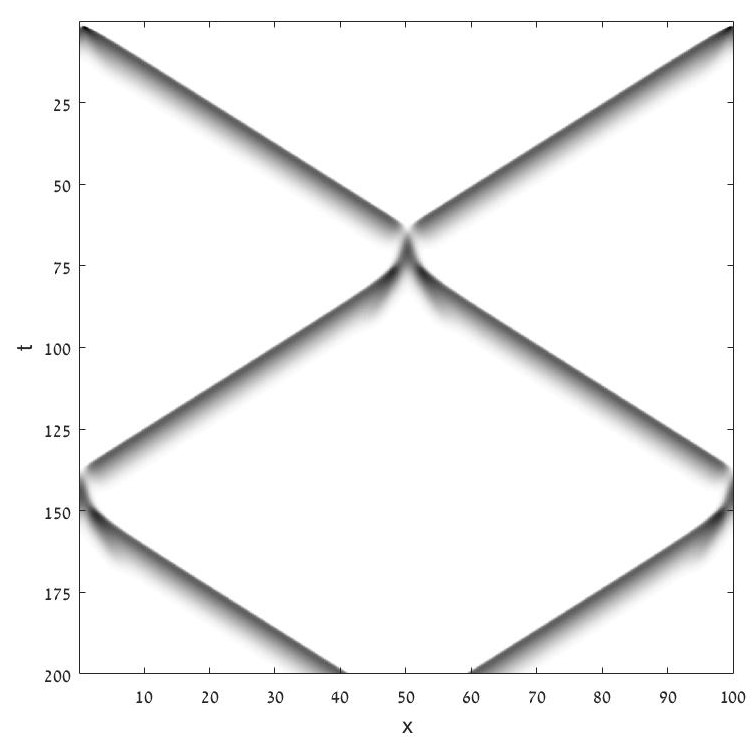
\includegraphics[scale=0.25]{a=9.5, 2.jpg}\hfill
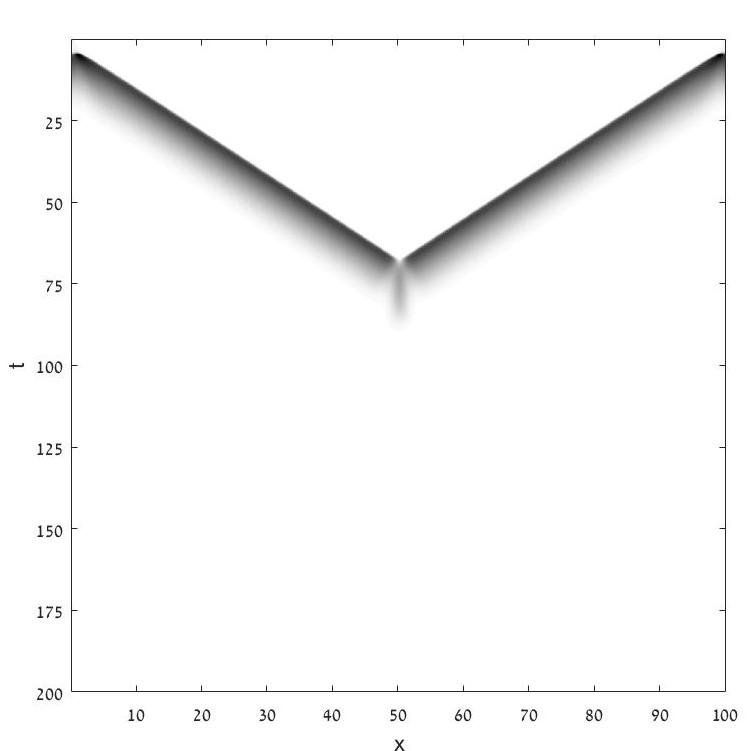
\includegraphics[scale=0.25]{a=9.5,dn=0,16, 2.jpg}\hfill
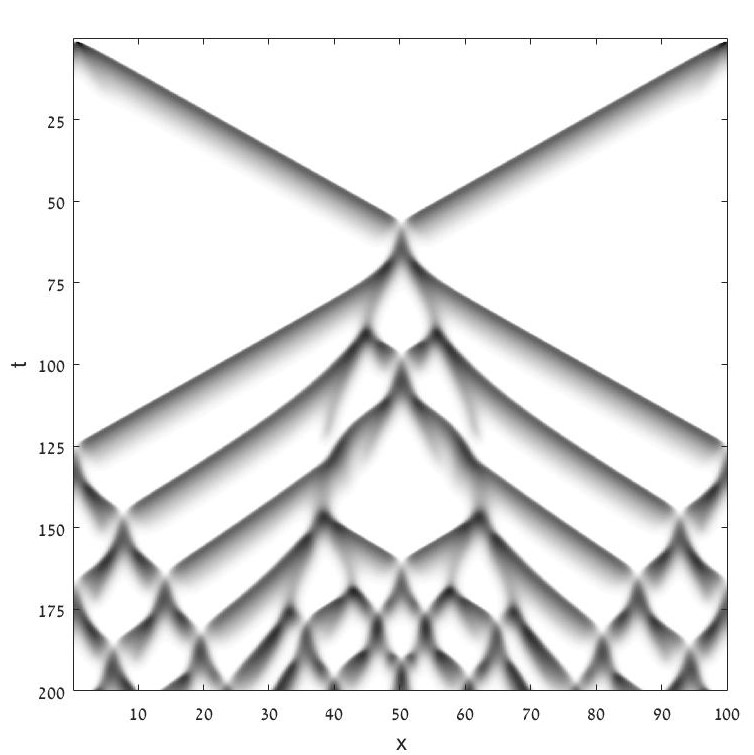
\includegraphics[scale=0.25]{a=10.4,dn=0,1, 2.jpg}
\caption{\label{im1}Space-time plots representing the polymerized actin filaments. A small linear perturbation was used as an initial condition. The difference between the three plots is a consequence of implementation of different parameters. In the left plot $D_N=0.1$ and the overall mass, $A=9.5$, In the center plot $D_N=0.16$, $A=9.5$ and in the right plot $D_N=0.1$ and $A=10.4$. Other common parameters are: $D_I=0.001$,$K_N=2$, $K_I=0.3$} 
\end{figure}

As seen from the results, changes in the overall mass and in the diffusion coefficient lead to three types of collisions: cross-over, annihilation and nucleation. Cross-over collision leads to a soliton-like behavior in which waves maintain their shapes and speed, while annihilation leads to dissipative behavior, which is more typical to dissipative systems [2]. Nucleation leads to the formation of new waves after collision in a self-similar way. This results lead to the understanding that there may be systems in which different collision patterns appear in accordance with different parameters. We would expect that in a system, such as cell membranes, that exhibits a wide range of parameters there would be different wave regimes that usually do not appear together. This result may lead to the expectation of a widespread occurrence of wave patterns in such systems.  
 
 \begin{figure}[hbt!]\centering
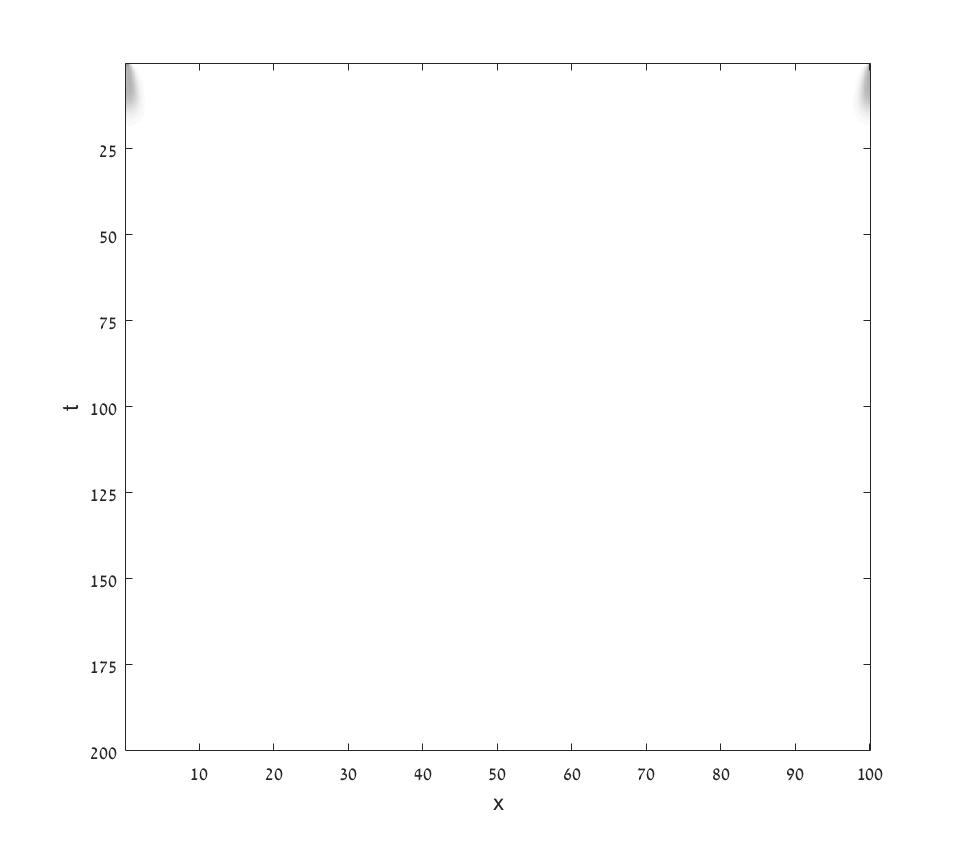
\includegraphics[scale=0.17]{a=9.5, dn=0.2.jpg}\hfill
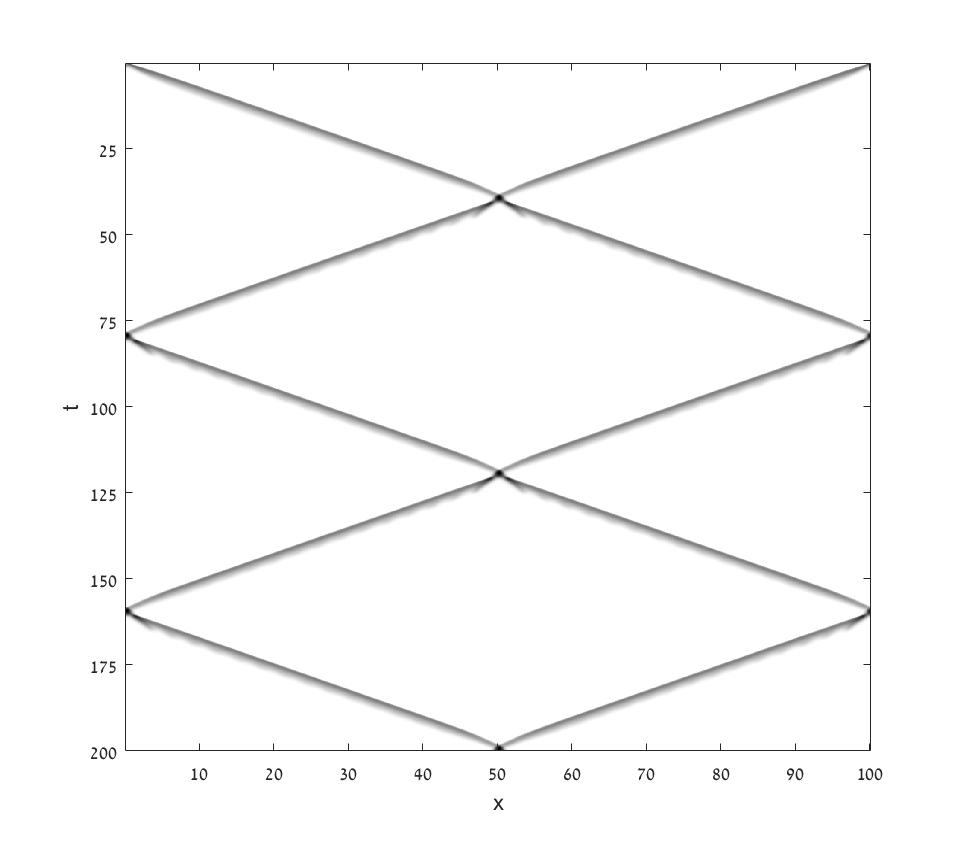
\includegraphics[scale=0.17]{a=9.5,dn=0.02.jpg}\hfill
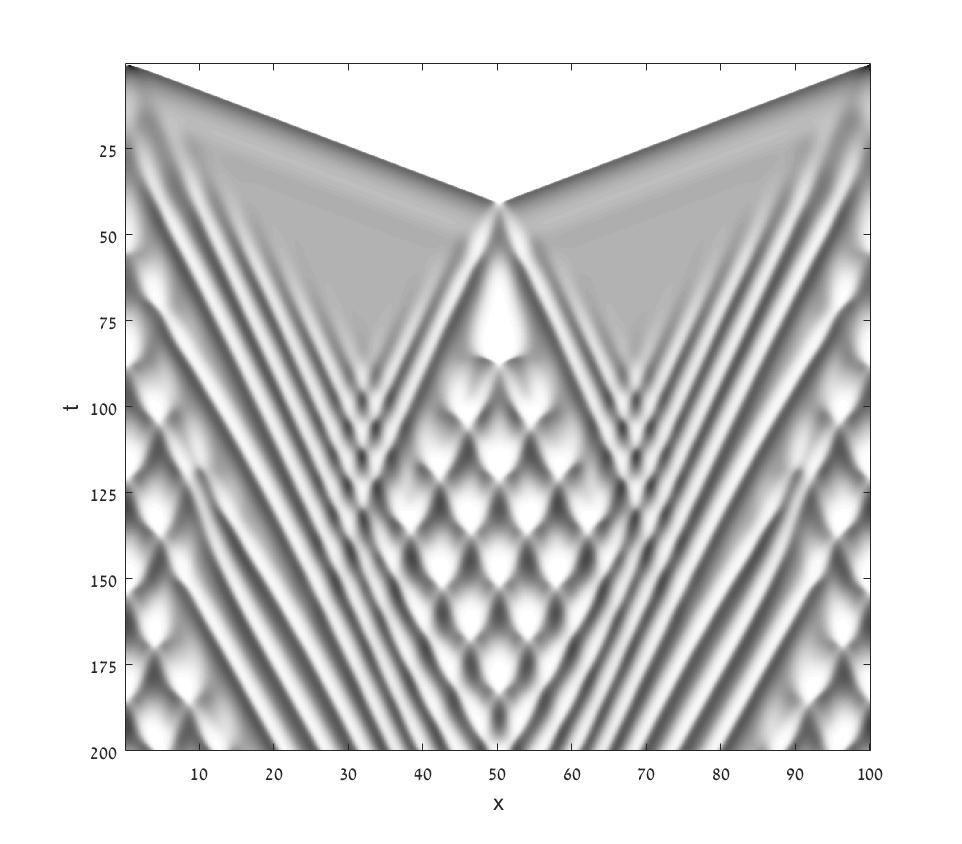
\includegraphics[scale=0.17]{a=13.5, dn=0.1.jpg}
\caption{\label{im1}Other pulse patterns that matches different parameter range. In the left plot we have used a diffusion coefficient of $D_N=0.2$ which leads to substantial diffusion right from the beginning and the dissipation of the pulse, in the center plot we have used $D_N=0.02$ which leads to a more localized pulse and a cross-over behavior and in the right plot we have used  $D_N=0.1$ and changed the mass to be $A=13.5$, which leads to a creation of wavelets and an aggressive nucleation pattern.} 
\end{figure}
\newpage
%%%%%%%%%%%%%%%%%%%%%%%%%%%%%%%%%%%%%%%%%%%%%%%%%%%%%%%%%%%%%%%%%%%%%%%%%%%%%%%%%%%%%%%%%%%%%%%%%%%%%%%%%
%%%%%%%%%%%%%%%%%%%%%%%%%%%%%%%%%%%%%%%%%%%%%%%%%%%%%%%%%%%%%%%%%%%%%%%%%%%%%%%%%%%%%%%%%%%%%%%%%%%%%%%%%
\sectA{Linear stability analysis}

In order to learn how to examine linear stability for nonuniform solutions numerically I took the solution  that I found to $(1)$ with $D_N=0.1$ and $A=9.5$, i.e. the right plot of FIG.2, as a case study and performed linear stability analysis to this solution. It is important to emphasize that, of course, pulses are linearly stable so this was done for academic purposes.

First of all, because the model deals with propagating pulses it is necessary to transform the frame of reference to the co-moving frame of the pulse. To do so we change the coordinates, defining a co-moving coordinate $\xi$:
\beq
\xi&=&x-ct
\eeq
Here, $x$ is the spatial coordinate, $c$ is the propagation speed of the pulse and $t$ is the time coordinate.

Now, the set of equations will become:
\begin{eqnarray}
      \frac{dN}{dt}&=&-N+\frac{N^2S}{1+I}+c\frac{dN}{d\xi}+D_N\frac{d^2N}{d\xi^2} \\\nonumber
     \frac{dS}{dt}&=&N-\frac{N^2S}{1+I}+c\frac{dS}{d\xi}+\frac{d^2S}{d\xi^2} \\\nonumber
      \frac{dI}{dt}&=&-K_II+K_NN+c\frac{dI}{d\xi}+D_I\frac{d^2I}{d\xi^2}
\end{eqnarray}

Let the equations be represented generally as:
\beq
\frac{d\bm{U}}{dt}&=&\bm{F(U)}
\eeq
using Taylor expansion around a fixed point, \bm{$U_0$}, will lead to:
\beq 
\bm{F(U)=F(U_0)+\left.J_F\right |_{U=U_0}\cdot(U-U_0)}+O((\bm{U-U_0})^2)
\eeq
Where $\bm{J_F}$ is the jacobian matrix of $\bm{F}$ with respect to $\bm{U}$. By definition $\bm{F(U_0)}=0$, therefore setting $\bm{\delta U=U-U_0}$ will result:
\beq
\frac{d(\bm{U_0+\delta U)}}{dt}&=&\frac{d\bm{(\delta U)}}{dt}=\left.\bm{J_F}\right.\bm{|_{U=U_0}}\cdot\bm{\delta U}
\eeq
This is an eigenvalue problem with the characteristic equation:
\beq
det[\left.\bm{J_F}\right.\bm{|_{U=U_0}}-\lambda\bm{I}]&=&0
\eeq
The general solution for this problem is:
\beq
\bm{U(t)=U_0+}\sum_{i=1}^{n} a_i\bm{v_i}e^{\lambda_it}
\eeq
Where $\bm{v_i}$ are the jacobian eigenvectors, $\lambda_i$ are the eigenvalues and $a_i$ are coefficients determined by the initial conditions.
Thus, in order to examine whether a solution is stable or not, it is sufficient to see if the real part of all of the eigenvalues is negative. This will lead to decaying solutions with time.

To implement this method into our model and examine whether or not the solution is stable we, first, need a steady-state solution to examine. We take the numerical solution we found to (1), at a time of $t=25$, and use it as our fixed point.
Next, we want to construct the jacobian numerically. The jacobian general form is:
%
\beq
J&=&\left (\begin{array}{c|c|c}
  \frac{\partial f_N}{\partial N} & \frac{\partial f_N}{\partial S} & \frac{\partial f_N}{\partial I} \\[1ex] \hline \frac{\partial f_S}{\partial N} & \frac{\partial f_S}{\partial S} & \frac{\partial f_S}{\partial I} \\[1ex] \hline \frac{\partial f_I}{\partial N} & \frac{\partial f_I}{\partial S} & \frac{\partial f_I}{\partial I} \end{array}\right )
\eeq
This jacobian is actually a nine block matrix, where each block represents the $\frac{\partial f_i}{\partial j}$ derivative. Using the discrete representation of the functions, where $i$ is the rows index, we acquire:
\beq
f_{N,i}&=&-N_i+\frac{N_i^2S_i}{1+I_i}+c\frac{N_{i+1}-N_{i-1}}{2\Delta\xi}+D_N\frac{N_{i+1}+N_{i-1}-2N_i}{\Delta\xi^2} \\\nonumber
f_{S,i}&=&N_i-\frac{N_i^2S_i}{1+I_i}+c\frac{S_{i+1}-S_{i-1}}{2\Delta\xi}+\frac{S_{i+1}+S_{i-1}-2S_i}{\Delta\xi^2} \\\nonumber
f_{I,i}&=&-K_II_i+K_NN_i+c\frac{I_{i+1}-I_{i-1}}{2\Delta\xi}+D_I\frac{I_{i+1}+I_{i-1}-2I_i}{\Delta\xi^2}
\eeq
We derive the functions with respect to the $j'th$ index, which is the columns index, to receive back the entries of the each block. To simplify the jacobian form we can separate the matrix into a sum of two matrices. One is the jacobian of the algebraic terms and the other is the jacobian of the $\xi$ derivatives. Thus, we can write:
\beq
J&=&J_{der}+J_{alg}
\eeq
Therefore, if we take, for instance, the $ \frac{\partial f_N}{\partial N}$ block it will have a tridiagonal form of:
\beq
\frac{\partial f_N}{\partial N}_{der}&=&\begin{pmatrix}
  \frac{-2D_N}{\Delta\xi^2} &  \frac{D_N}{\Delta\xi^2}+\frac{c}{2\Delta\xi} & 0 & \cdots&0&\frac{D_N}{\Delta\xi^2}-\frac{c}{2\Delta\xi}  \\[1ex] \frac{D_N}{\Delta\xi^2}-\frac{c}{2\Delta\xi}&\frac{-2D_N}{\Delta\xi^2} & \frac{D_N}{\Delta\xi^2}+\frac{c}{2\Delta\xi} & 0 & \vdots&0\\[1ex] 0 & \ddots & \ddots & \ddots &  0&\vdots\\[1ex]\vdots&\cdots&\ddots&\ddots&\ddots\\[1ex] \frac{D_N}{\Delta\xi^2}+\frac{c}{2\Delta\xi}&0&\cdots& &\frac{D_N}{\Delta\xi^2}-\frac{c}{2\Delta\xi}&\frac{-2D_N}{\Delta\xi^2} & \end{pmatrix} 
 \eeq
 \beq
 \nonumber
  \frac{\partial f_N}{\partial N}_{alg}&=&\begin{pmatrix}
  \frac{2N_1S_1}{1+I_1-1} &  0 & \cdots&0  \\[1ex] 0&\frac{2N_2S_2}{1+I_2-1} &0 & \cdots&0\\[1ex] & \ddots & \ddots & \ddots &  \\[1ex] 0&\cdots&0&\frac{2N_nS_n}{1+I_n-1}\end{pmatrix}
\eeq
\beq
\nonumber
\frac{\partial f_N}{\partial N}=\frac{\partial f_N}{\partial N}_{der}+\frac{\partial f_N}{\partial N}_{alg}
\eeq
%
It is important to notice that we implemented periodic boundary conditions to each block:
\beq
\left[\frac{\partial f_N}{\partial N}\right]_{1,n}&=&\left[\frac{\partial f_N}{\partial N}\right]_{1,0}\\\nonumber \left[\frac{\partial f_N}{\partial N}\right]_{n,1}&=&\left[\frac{\partial f_N}{\partial N}\right]_{n,n+1}
\eeq
This is because we have used periodic boundary conditions to solve (1). Without applying these boundary conditions we would get eigenvalues and eigenvectors that do not reflect the correct stability of the solution. 

In a similar manner each block is constructed and builds up the jacobian matrix. To find the eigenvalues and eigenvectors of the jacobian we can use different algorithms which will not be disscussed in this report. 

\begin{figure}[hbt]\centering
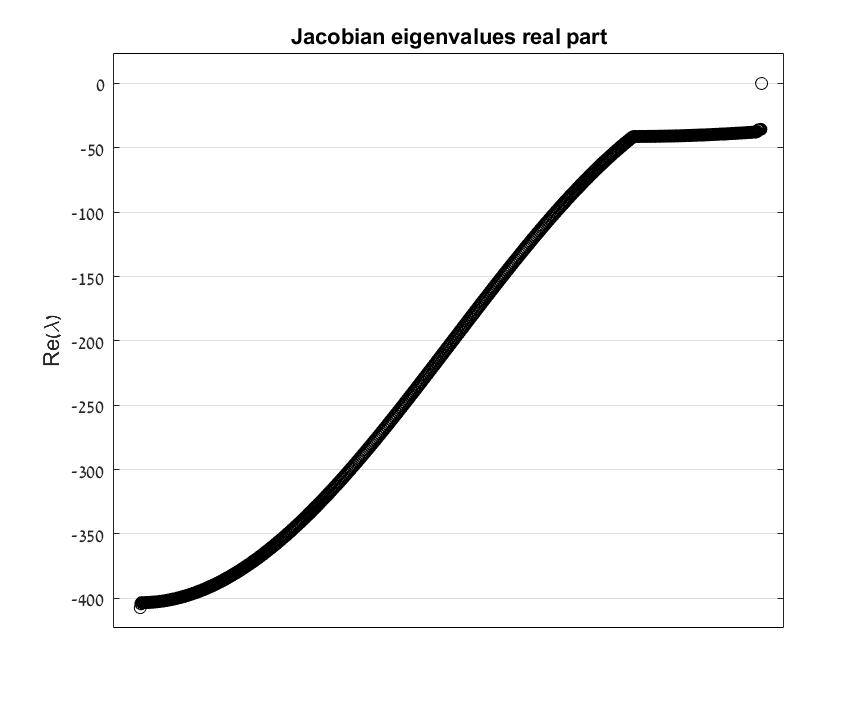
\includegraphics[scale=0.22]{eigenvalues of N.jpg}
\caption{\label{im1}The jacobian matrix eigenvalues real part. The single neutral eigenvalue is prominent with respect to the other eigenvalues.} 
\end{figure}
As can be seen from the plot, all of the eigenvalues we found are negative, apart from a single neutral eigenvalue $\lambda=0$. This eigenvalue is typical for a mass-conservation system and give rise to all of the phenomenons that we discussed in the previous section. Examination of the corresponding eigenfunctions reveals a localized behavior that matches the soliton-like behavior that was expected.

If we change the propagation speed to be inaccurate we will see a change in the eigenvalues, as follows from the figure:

\begin{figure}[hbt]\centering
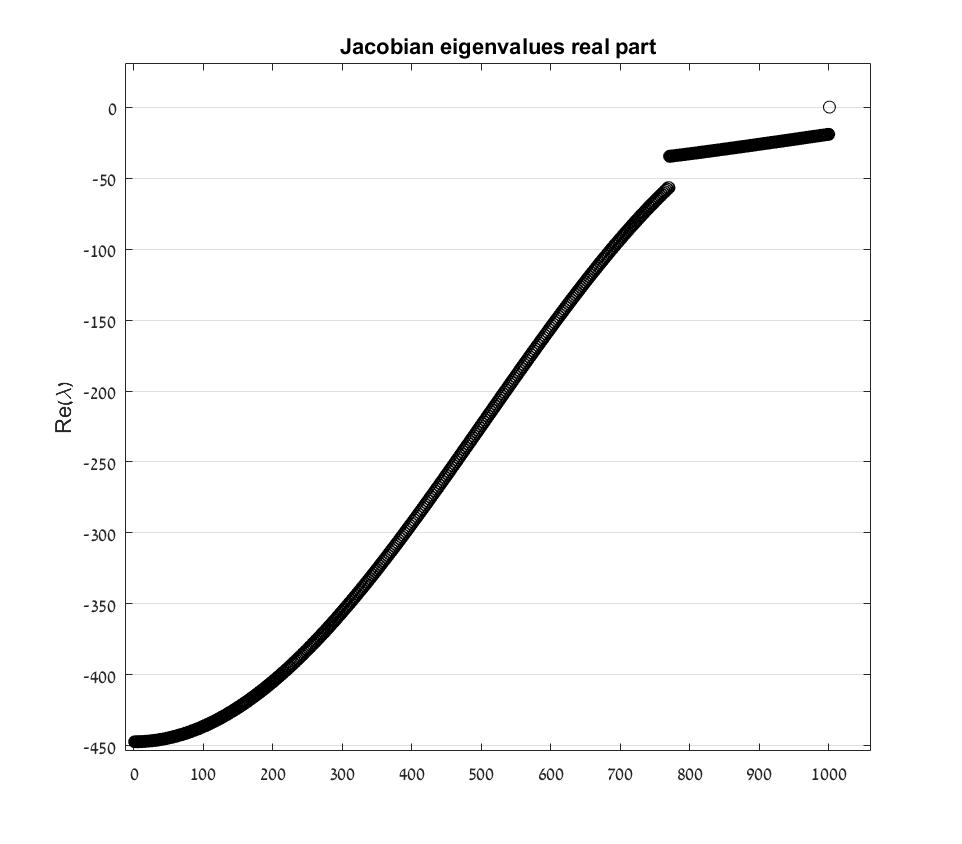
\includegraphics[scale=0.20]{c=c+10.jpg}
\caption{\label{im1}The jacobian matrix eigenvalues real part with the pulse propagation speed increased by 10 units. There is a change in the range of the eigenvalues, as well as the distribution of the eigenvalues. Nevertheless, the neutral eigenvalue still exists.} 
\end{figure}
\newpage
\begin{figure}[hbt]\centering
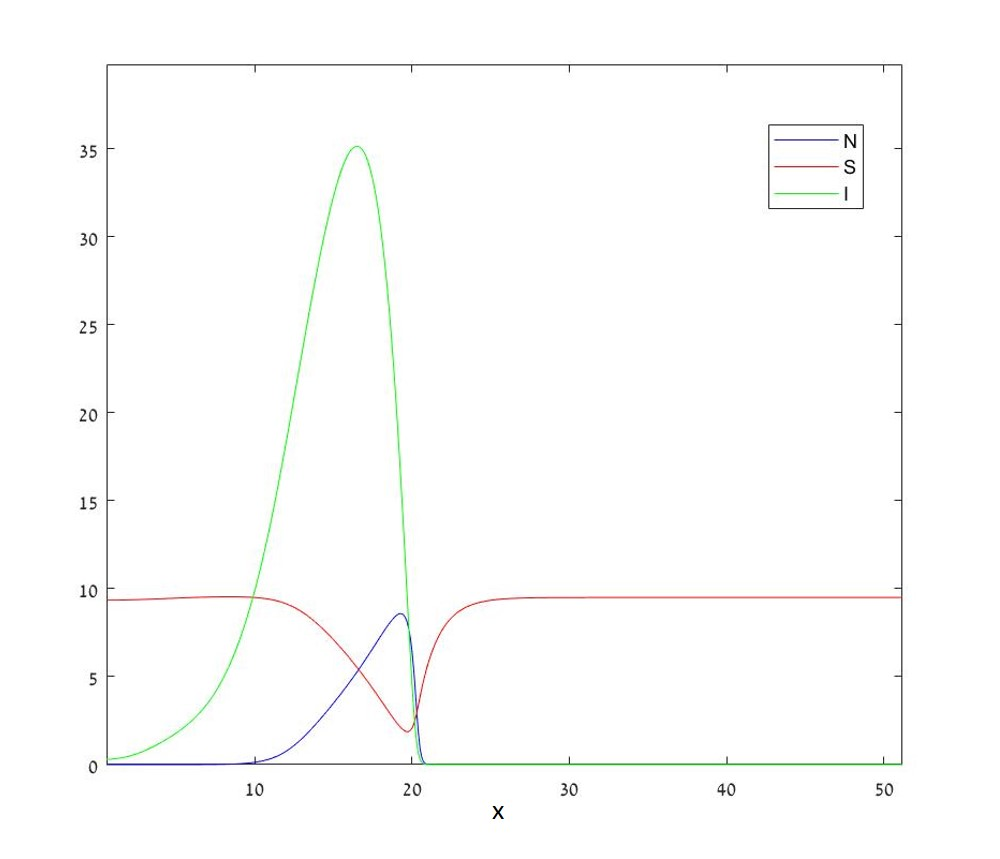
\includegraphics[scale=0.45]{typsol.jpg}
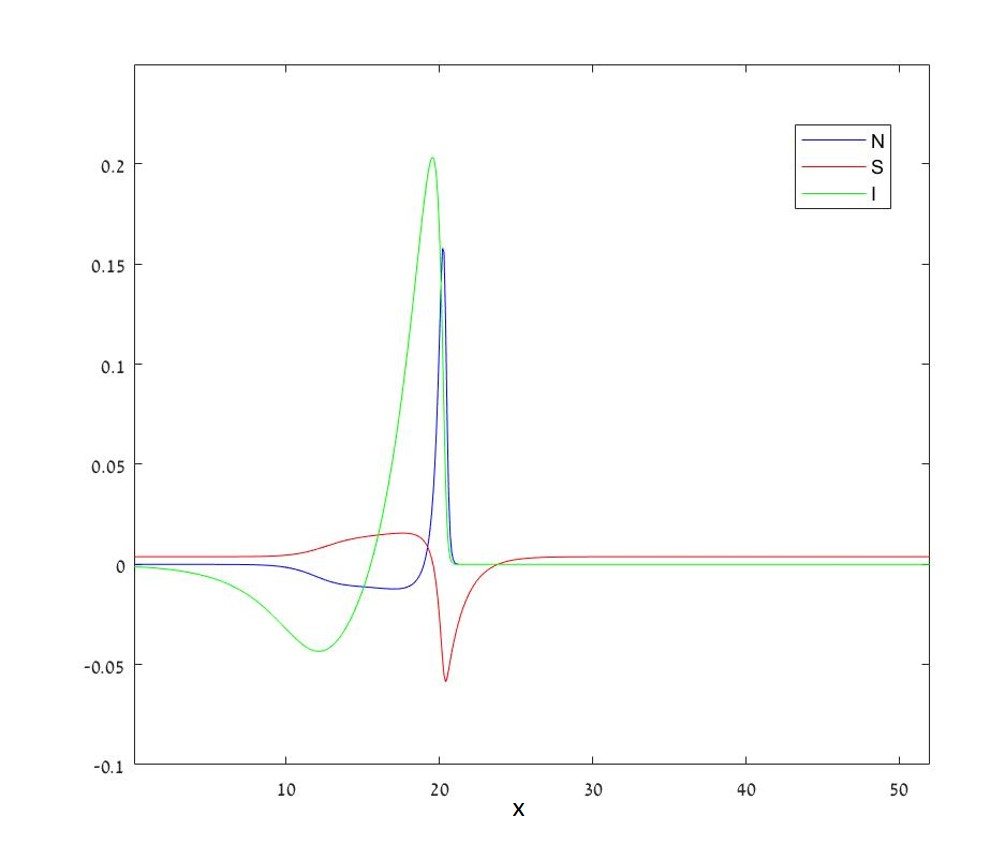
\includegraphics[scale=0.45]{eigenfun.jpg}
\caption{\label{im1}A steady-state solution to (1) at time of $t=25$ with $A=9.5, D_N=0.1$ (left), and the eigenfunctions that correspond to the neutral eigenvalue of this solution (right). As can be seen This eigenfunctions are localized and not oscillatory.} 
\end{figure}

%%%%%%%%%%%%%%%%%%%%%%%%%%%%%%%%%%%%%%%%%%%%%%%%%%%%%%%%%%%%%%%%%%%%%%%%%%%%%%%%%%%%%%%%%%%%%%%%%%%%%%%%%
\sectA{Summary}

In this project we examined a simplified, one-dimensional, reaction-diffusion model that describes the process of actin polymerization. The model consists of a set of parabolic nonlinear partial differential equations which we solved using the forward Euler method. It was important to keep the space and time steps sufficiently small in order to acquire a stable solution and fulfill the stability criterion. Nevertheless, we had limited computation resources, therefore it was also important to build an efficient algorithm.

The results led to three different kinds of collisions between pulses: cross-over, which indicates a soliton-like behavior, annihilation which indicates a dissipative behavior, and nucleation of new pulses. The diversity of collisions is an outcome of changes in the overall mass parameter and of the diffusion coefficient of the polymerized actin. From this result we can assume that systems which exhibit a wide range of parameters may reveal different collision patterns together. Beyond these results, changes of the wave profiles were also acquired with the changes of the mass and the diffusion parameters. Large diffusion led to the dissipation of the wave from the beginning, small diffusion led to a more localized pulse and larger mass triggered wavelets and nucleation.   

For academic purposes we have used the cross-over solution as a case study for linear stability analysis. We have transformed to the co-moving frame of the pulse using its propagation speed and constructed the jacobian matrix corresponding the model equations. It was especially important to implement the correct boundary conditions to the matrix, otherwise we would get wrong stability analysis. The real part of all of the eigenvalues turned to be negative, as expected, apart from a single neutral eigenvalue. The eigenfunction that corresponded to this neutral eigenvalue appeared to be localized, in a similar way as the general solution, in agreement with the soliton behavior that we have encountered.   

%%%%%%%%%%%%%%%%%%%%%%%%%%%%%%%%%%%%%%%%%%%%%%%%%%%%%%%%%%%%%%%%%%%%%%%%%%%%%%%%%%%%%%%%%%%%%%%%%%%%%%%%%
\sectA{References}

[1] E. Bernitt, H.-G. D$\ddot{o}$bereiner, N. S. Gov, and A. Yochelis,
Nature Communications 8, 15863 (2017).

[2] A. Yochelis, C. Beta, and N. S. Gov, Phys. Rev. E 101, 022213 (2020)

[3] C. Beta, and N. S. Gov, and A. Yochelis, Cells 9, 1533 (2020)

[4] W.H. Press, S.A. Teukolsky, W.T. Vetterling, B.P. Flannery, "Numerical Recipes in C: The Art of Scientific Computing" Second Edition (Cambridge University Press, 1992)

[5] S.H. Strogatz, "Nonlinear Dynamics and Chaos: with Applications to Physics, Biology, Chemistry and Engineering", (Addison-Wesley, Reading Mass, 1994)

%%%%%%%%%%%%%%%%%%%%%%%%%%%%%%%%%%%%%%%%%%%%%%%%%%%%%%%%%%%%%%%%%%%%%%%%%%%%%%%%%%%%%%%%%%%%
\end{document} 
